\documentclass{exam}
\usepackage[utf8]{inputenc}
\usepackage[T1]{fontenc}
\usepackage{amsmath,amsfonts,amsthm} % Math packages for equations
\usepackage{tikz}
\usepackage{hyperref}
\usepackage{url}

\DeclareMathOperator{\diff}{d}
\DeclareMathOperator{\sign}{sgn}
\DeclareMathOperator*{\Res}{Res}
\DeclareMathOperator*{\reg}{reg}
\DeclareMathOperator*{\Ai}{Ai}
\DeclareMathOperator*{\Bi}{Bi}
\newcommand{\calB}{\mathcal{B}}
\newcommand{\calL}{\mathcal{L}}

\title{Lectures on Resurgence and Trans-Series}
\author{Marco Knipfer, University of Alabama}
\date{Week 10, Version: \today}

\begin{document}
\maketitle

\begin{questions}
    \setcounter{question}{9}
    \question (\textbf{The Airy Equation: Integral})\\
    In this exercise we focus on the integral represenation of the Airy equation.
    We will find the asymptotic expansion like in the last exercise.
    Later (not on this exercise sheet) we will also be able
    to see how the Stokes phenomenon appears because the path of steepest descent deforms as
    we change $x$.

    The integral in question is
    \begin{equation}
        I_\gamma = \frac{1}{2 \pi i} \int_\gamma \diff\! z\, e^{S(z)}\,,\quad x z - \frac{z^3}{3}\,,
    \end{equation}
    where $\gamma$ is some path in $\mathbb{C}$.

    \begin{parts}
        \part (\textbf{Possible curves $\gamma$})\\
        \label{part:endpoints}
        Let us write $z = \rho e^{i\phi}$.
        Find out for which ``endpoints at infinity'' in $\mathbb{C}$ the integral converges.
        For that you have to find out in what regions (which $\phi$) $\Re(S(z))<0$ as $\rho \to \infty$.
        \part (\textbf{Connection to the Airy equation})\\
        Show that the integral $I_\gamma(x)$ fulfills the Airy equation
        \begin{equation}
            y''(x) = x y(x)\,,
        \end{equation}
        if the integrand vanishes at the end points, \emph{i.e.}\ the end points at infinity
        are in the reagions calculated in~(\ref{part:endpoints}).
        
        \textsc{Tipp:} No integration by parts needed, just have to see it.
        If you don't see it, calculate $S'(z)$.
        
        \part (\textbf{Three paths not independent})\\
        Three possible paths connecting the areas calculated in~(\ref{part:endpoints}) are
        shown in Figure~\ref{fig:contours}.
        Explain why only two of them are independent.
        \begin{figure}[tbh]
            \centering
            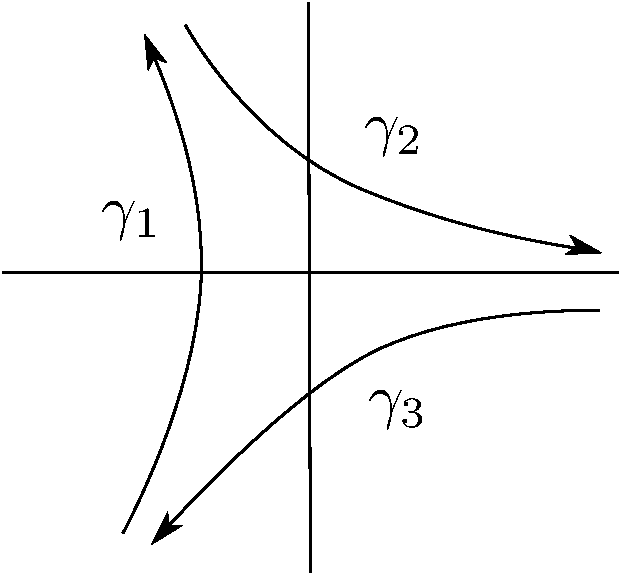
\includegraphics[width=0.3\textwidth]{airycontours.pdf}
            \caption{Three allowed contours leading to solutions to the Airy equation.
            Figure from  \url{http://arxiv.org/abs/1206.6272}}
            \label{fig:contours}
        \end{figure}

        \part (\textbf{Transformation of the integral})\\
        From now on we will focus on the contour $\gamma_1$ since it will give us the Airy function
        $\Ai(x)$.
        Show that the substitutions 
        \begin{align}
            z &= u r^{\frac{1}{2}}\\
            x &= r e^{i \kappa}
        \end{align}
        give
        \begin{align}
            \Ai(x) &= \frac{\sqrt{r} }{2 \pi i}\int_{\gamma_1} \diff\!u\, e^{r^{3 / 2} (e^{i \kappa} u - \frac{u^3}{3})}
            = \frac{\sqrt{r} }{2 \pi i}\int_{\gamma_1} \diff\!u\, e^{r^{3 / 2} S_\kappa(u)}\,,\\
            S_\kappa(u) &= e^{i \kappa}u - \frac{u^3}{3}\,.
        \end{align}
        Note that we have removed the $r$-dependence from the stationary points of the exponent.
        \part (\textbf{Saddle point method: Curve of steepest descent})\\
        Find the two saddle points $u^{\text{R, L}}$ of $S_\kappa$ and their actions $S_\kappa(u^{\text{R,L}})$.
        Explain how they move as we change $\kappa$.

        Let's first focus on $x\in\mathbb{R}$, \emph{i.e.}\ $\kappa = 0$ and the saddle point $u^{\text{L}}$ (the negative one).
        The curve $\gamma^\text{L}_\kappa$ ($\kappa = 0$) of steepest descent through that point $u^{\text{L}}$ is also the curve of constant imaginary part of the action,
        \begin{equation}
            \Im[S(u) - S(u^{\text{L}})] = 0\,.
            \label{eq:constIm}
        \end{equation}
        Write $u=a + ib$ and determine $b(a)$ from~(\ref{eq:constIm}).
        You should find a courve that looks like $\gamma_1$ and is given by
        \begin{equation}
            b(a) = \pm \sqrt{3} (a^2 - 1)^{\frac{1}{2}}\,,\quad a<-1\,.
        \end{equation}
        
        Check that for large $a$ the curve $\gamma^\text{L}_0$ stays in the allowed region such that $I_\gamma$ converges,
        \begin{equation}
            - \frac{\pi}{6} + \frac{2}{3}\pi n < \phi < \frac{\pi}{6} + \frac{2}{3} \pi n\,,\quad n \in \{ 0,1,2 \}\,,
        \end{equation}
        and that the curve $\gamma^\text{L}_0$ goes through the saddle point $u^\text{L}$.
        We thus have a curve that has the same ``end points'' as $\gamma_1$ and we can deform $\gamma_1$ to
        $\gamma^\text{L}_0$.

        \part ({Saddle point method: Laplace's Method, zeroth order})\\
        Laplace's method (Bender 6.4) for an integral of the form
        \begin{equation}
            I(x) = \int_a^b \diff\!t\, f(t) e^{x S(t)}\,,
        \end{equation}
        gives if $c$ is the maximum of $S(t)$, $c\in(a,b)$,
        \begin{equation}
            I(x) \sim \frac{\sqrt{2\pi} f(c) e^{x S(c)} }{\sqrt{-x S''(c)} }\,,
        \end{equation}
        if $f(c)\neq 0$.
        Since our $S(u)$ along the curve $\gamma^\text{L}_0$ has its maximum at $u^\text{L}$ we can
        use Laplace's method (note: $f=1$ here).

        Show that Laplace's method for the integral along the curve $\gamma^\text{L}_0$ gives the
        zeroth order of the asymptotic expansion of $\Ai$ (see exercise sheet of week 9),
        \begin{equation}
            Z_{\Ai}(x) = \frac{1}{2 \sqrt{\pi} x^{1 / 4}} e^{\frac{2}{3} x^{3 / 2}}\sum_{n=0}^{\infty} (-1)^2 a_n x^{- \frac{3}{2}n}\,.
        \end{equation}

        Note that for the zeroth order of the expansion didn't even need the parametrization of the curve,
        but it will still be useful!
        
        \textsc{Bonus:} Determine the higher orders and show that they are the same as in $Z_{\Ai}$, see
        \emph{e.g.}\ Bender p.\ 272. 
        
    \end{parts}

    
    
\end{questions}


\end{document}
